\documentclass[tikz, svgnames]{standalone}
\usetikzlibrary{mindmap}
\begin{document}
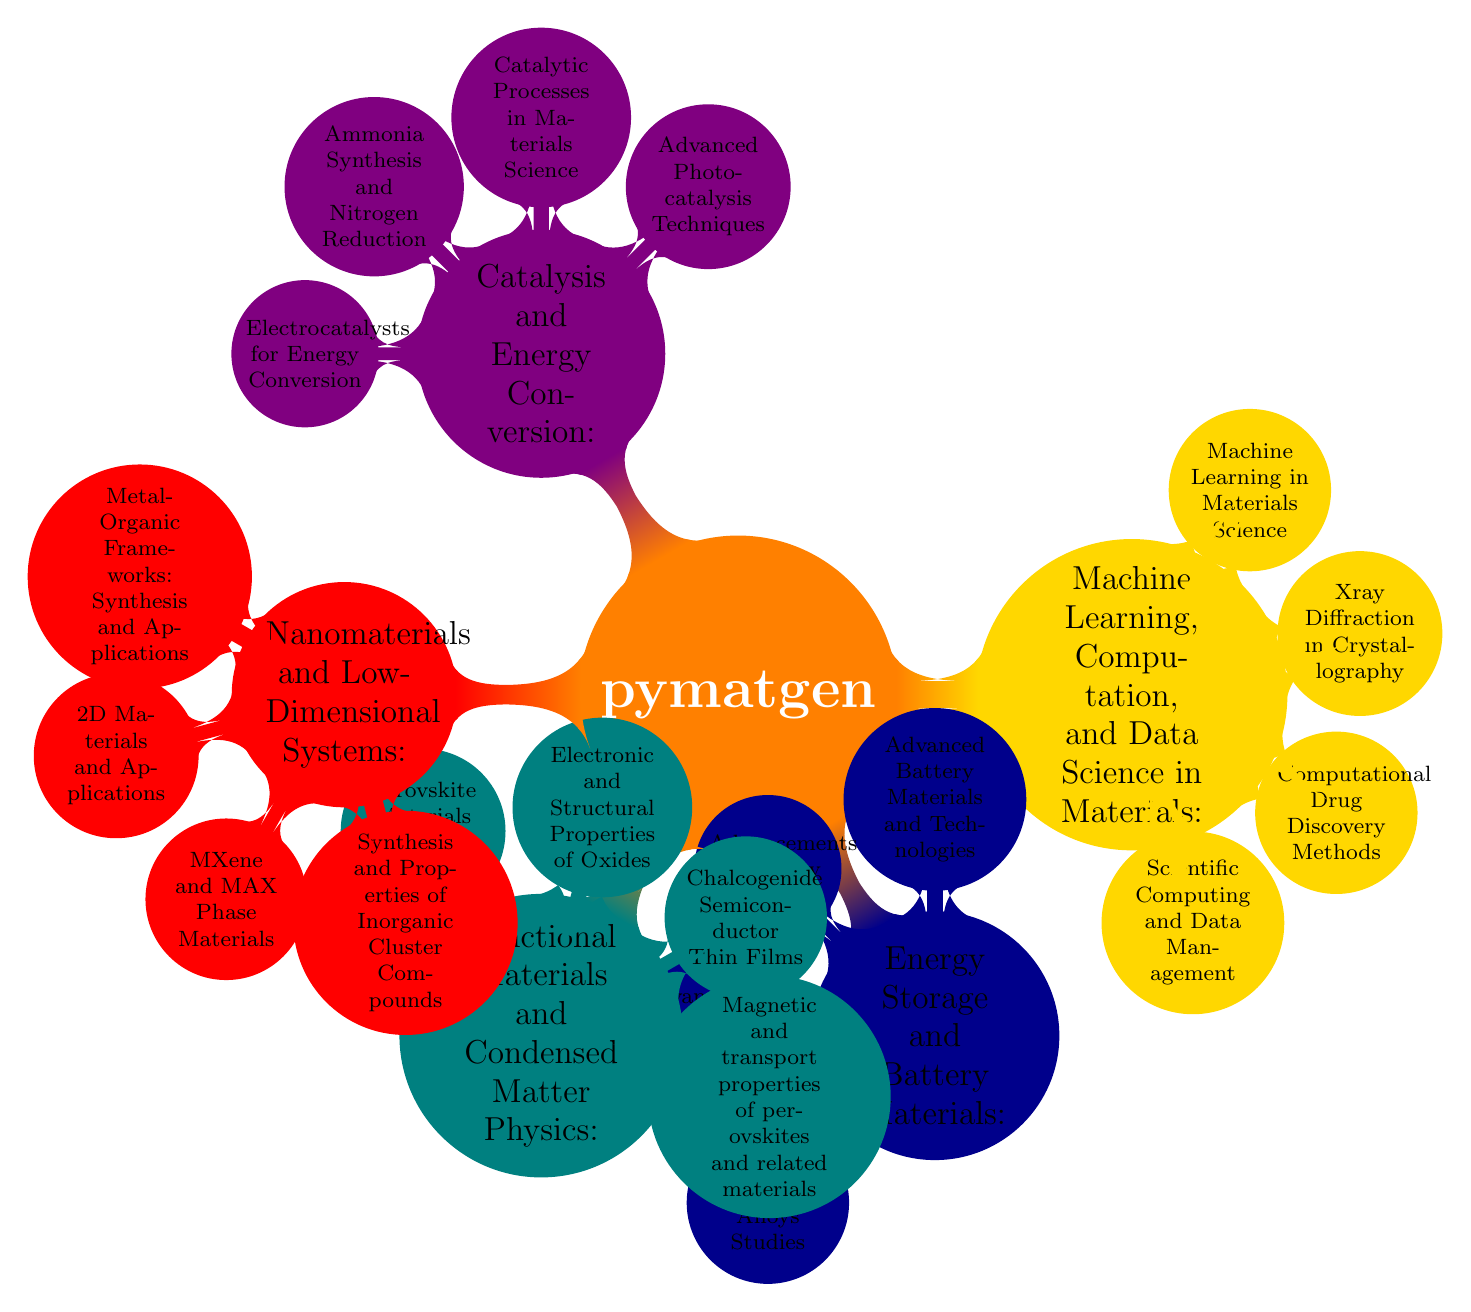
\begin{tikzpicture}[
    mindmap, every node/.style=concept, concept color=orange, text=white,
    level 1/.append style={level distance=5cm, sibling angle=60, font=\large},
    level 2/.append style={level distance=3cm, sibling angle=45}
  ]

  \node{\textbf{\huge{pymatgen}}} [clockwise from=0]
  child [concept color=Gold, text=black] {
      node {Machine Learning, Computation, and Data Science in Materials:} [clockwise from=60]
      child { node {Machine Learning in Materials Science} }
      child { node {X\-ray Diffraction in Crystallography} }
      child { node {Computational Drug Discovery Methods} }
      child { node {Scientific Computing and Data Management} }
    }
  child [concept color=DarkBlue, text=black] {
      node {Energy Storage and Battery Materials:} [counterclockwise from=90]
      child { node {Advanced Battery Materials and Technologies} }
      child { node {Advancements in Battery Materials} }
      child { node {Advancements in Solid Oxide Fuel Cells} }
      child { node {High Entropy Alloys Studies} }
    }
  child [concept color=Teal, text=black] {
      node {Functional Materials and Condensed Matter Physics:} [clockwise from=120]
      child { node {Perovskite Materials and Applications} }
      child { node {Electronic and Structural Properties of Oxides} }
      child { node {Chalcogenide Semiconductor Thin Films} }
      child { node {Magnetic and transport properties of perovskites and related materials} }
    }
  child [concept color=Red, text=black] {
      node {Nanomaterials and Low-Dimensional Systems:} [counterclockwise from=150]
      child { node {Metal\-Organic Frameworks: Synthesis and Applications} }
      child { node {2D Materials and Applications} }
      child { node {MXene and MAX Phase Materials} }
      child { node {Synthesis and Properties of Inorganic Cluster Compounds} }
    }
  child [concept color=Purple, text=black] {
      node {Catalysis and Energy Conversion:} [clockwise from=180]
      child { node {Electrocatalysts for Energy Conversion} }
      child { node {Ammonia Synthesis and Nitrogen Reduction} }
      child { node {Catalytic Processes in Materials Science} }
      child { node {Advanced Photocatalysis Techniques} }
    }
;
\end{tikzpicture}
\end{document}
